\section{Materials and methods}
\label{sec:method}

\subsection{Data}
\label{sub:data}
We train our model on the MNIST dataset \cite{MNIST} consisting of 70000 i.i.d. $28 \times 28$ pixel images of handwritten digits in black and white, $\vec{X} = \set{\vec{X}\order{i}}^N_{i=1}$. We use a training set of 60000 images including the validation set and evauluate the performance on reconstructions of the 10000 images test set. 
For i.i.d. data like this, each pixel are assumed to follow a marginal joint probability distribution, which makes it possible to decompose the log-likelihood of each datapoint, $i$, in a sum:
\begin{equation}
	\log \dec{\vec{X}} = \log \dec{\vec{X}\order{1}, ..., \vec{X}\order{N}} = \sum^N_{i=1} \log \dec{\vec{X}\order{i}} 
\end{equation}are 
Generalizing the VAE model from a single image to all, we write $\vec{x} = \vec{X}\order{i}$ for uncluttered and simple notation in the following equations.

\subsection{Model}
\label{sub:the_model}

\begin{figure*}
	\centering
	\usetikzlibrary{positioning}
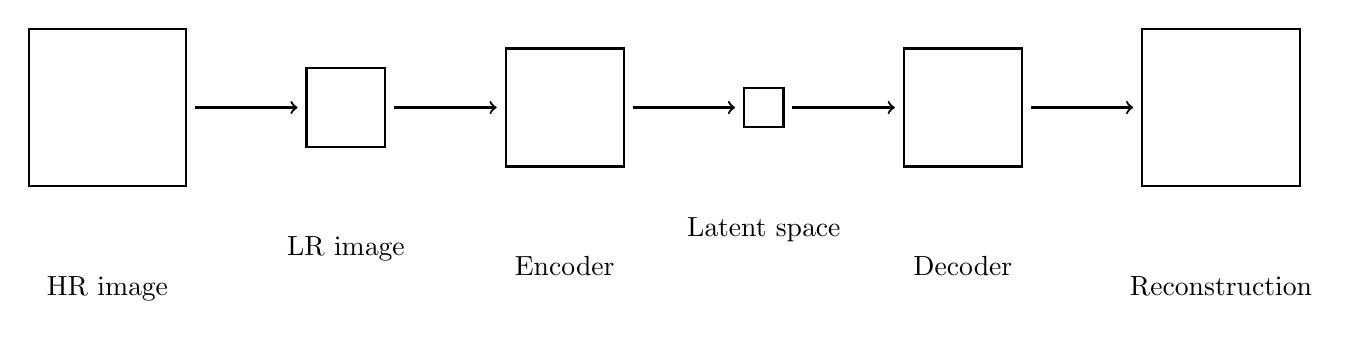
\begin{tikzpicture}[x = 1cm, y = 1cm, thick,
		image/.style={rectangle, draw, inner sep = 0pt, minimum size = 2 cm},
		network/.style={rectangle, draw, inner sep = 0pt, minimum size = 2 cm},
		arrow/.style={ ->, shorten <= 1 mm, shorten >= 1 mm}
	]
	
	\node[image, minimum size = 2 cm] (HR) at (0, 0) {};
	\node[below = of HR] {HR image};
	
	\node[image, minimum size = 1 cm, right = 1.5 cm of HR] (LR) {};
	\node[below = of LR] {LR image};
	
	\node[network, minimum size = 1.5 cm, right = 1.5 cm of LR] (encoder) {};
	\node[below = of encoder] {Encoder};
	
	\node[network, minimum size = 0.5 cm, right = 1.5 cm of encoder] (latent) {};
	\node[below = of latent] {Latent space};
	
	\node[network, minimum size = 1.5 cm, right = 1.5 cm of latent] (decoder) {};
	\node[below = of decoder] {Decoder};
	
	\node[image, minimum size = 2 cm, right = 1.5 cm of decoder] (reconstruction) {};
	\node[below = of reconstruction] {Reconstruction};
	
	\draw[arrow] (HR) -- (LR);
	\draw[arrow] (LR) -- (encoder);
	\draw[arrow] (encoder) -- (latent);
	\draw[arrow] (latent) -- (decoder);
	\draw[arrow] (decoder) -- (reconstruction);
	
\end{tikzpicture}

	\caption{Diagram of model. Originals, $\vec{x}\idx{HR}$, are binarised and downsampled, $\vec{x}\idx{LR}$. Reconstructions, $\tilde{\vec{x}}\idx{HR}$, are they results of the VAE.}
	\label{fig:diagram}
\end{figure*}

To test the performance and robustness of a VAE when in lack of variables, which is the case for a SR-task, we made a model as seen in \ref{fig:diagram}. It is generating HR images, $\tilde{\vec{x}}_{HR}$ as close to the binarised original images $\vec{x}_{HR}$ from downsampled LR images $\vec{x}_{LR}$. $\vec{x}_{HR}$ are binarised using Bernoulli sampling and then downsampled to $\vec{x}_{LR}$ by a factor of $d$ using a mean filter (pooling layer).

\subsubsection{Variational auto-encoder}
\label{ssub:vae}
The VAE make reconstructions from a underlying probalistic data generating process inferring the same structure between similar digits. The similarity lies in the latent space, $\vec{z}$, which is here the stochastic layer seen in the center of the model. 

The input $\vec{x}_{LR}$ is mapped to the latent space through the encoder sampling from a normal distribution
$\vec{z} \sim \enc{\vec{z}|\vec{x}} = \mathcal{N}\parens{ \vec{z}|\vec{\mu}_\phi(\vec{x}),\vec{\sigma}^2_\phi(\vec{x})}$, where $\enc{\vec{z}|\vec{x}}$ is a variational approximation to the intractable true posterior $\dec{\vec{z}|\vec{x}}$. 

Given the sampled $\vec{z}$ the decoder can generate a reconstruction $\tilde{\vec{x}}_{HR}$, where each pixel are assumed to be drawn from a Bernoulli distribution $\vec{x} \sim \dec{\vec{x}|\vec{z}}=\mathcal{B}\parens{ \vec{x}|\vec{\mu}_\theta(\vec{z})}$ for binarised $\vec{x}$ (our case) or from a normal distribution $\vec{x} \sim \dec{\vec{x}|\vec{z}}=\mathcal{N}\parens{ \vec{x}|\vec{\mu}_\theta(\vec{z}),\vec{\sigma}^2_\theta(\vec{z})}$ for continuous $\vec{x}$ like f.ex. face images.

The neural networks (NN) output the distribution parameters $\vec{\mu}_\phi(\vec{x})$ and $\vec{\sigma}^2_\phi(\vec{x})$ for the variational approximation $\enc{\vec{z}|\vec{x}}$ and $\vec{\mu}_\theta(\vec{z})$ for the conditional generative Bernoulli distribution $\dec{\vec{x}|\vec{z}}$. 

This is model selection by drawing the best fitting distribution from a family of distributions and the main idea behind variational Bayesian inference as used by \cite{Kingma2013}. 
 
The marginal log-likelihood can be decomposed like for the EM-algorithm and variational inference \cite[\S10.2]{Bishop2006}:
To learn the models variational parameters $\phi$ and generative parameters $\theta$ jointly we obtain a per-pixel training criterion from the variational lower bound $\mathcal{L}\left(\vec{\theta},\vec{\phi};\vec{x}\right)$ derived from the mean-field approximation to the marginal log-likelihood:
\begin{equation}
	\log \dec{\vec{x}} = D_{KL}\left( \enc{\vec{z}|\vec{x}}||\dec{\vec{z}|\vec{x}}\right) + \mathcal{L}\left(\vec{\theta},\vec{\phi};\vec{x}\right)
\end{equation} 
Here the first term is the Kullback-Leibler divergence, which is a non-negative entropy measure of how much the 2 distributions differ.
\begin{equation}
	D_{KL}\left( \enc{\vec{z}|\vec{x}}||\dec{\vec{z}|\vec{x}}\right) = \int \enc{\vec{z}|\vec{x}} \log \curlies*{ \frac{\dec{\vec{x}|\vec{z}}}{\enc{\vec{z}|\vec{x}} } } \D{\vec{z}}
\end{equation}

Since the KL-divergence is non-negative the second term (``free energy'') works as a variational lower bound and follows the inequality:

\begin{gather}
	\begin{split}
		\log \dec{\vec{x}} & \ge \mathcal{L}\left(\vec{\theta},\vec{\phi};\vec{x}\right)
		\\ & =
		\int \enc{\vec{z}|\vec{x}} \log \curlies*{ \frac{\dec{\vec{x},\vec{z}}}{\enc{\vec{z}|\vec{x}} } } \D{\vec{z}} \\ 
		& = \E_{\enc{\vec{z}|\vec{x}}} \brackets{- \log \enc{\vec{z}|\vec{x}} + \log \dec{\vec{x},\vec{z}} } 
		\\
		& = -D_{KL}\parens{ \enc{\vec{z}|\vec{x}}||\dec{\vec{z}} } 
		\\ 
		& \quad+ \E_{\enc{\vec{z}|\vec{x}}} \brackets{\log \dec{\vec{x}|\vec{z}} }   	
	\end{split} 
\end{gather}

\change{Rewrite this to text.}
\begin{itemize}
		\item The \textbf{first term} is the \textbf{regularisation} for $\vec{\phi}$ keeping the approximate posterior $\enc{\vec{z}|\vec{x}}$ close to the prior $\dec{\vec{z}}$. It has a differentiable analytical solution.
		\item The \textbf{second term} is the expected negative \textbf{reconstruction error}. This has a differentiable Monte Carlo estimate:
		\begin{equation*}
			\E_{\enc{\vec{z}|\vec{x}}} \brackets{\log \dec{\vec{x}|\vec{z}} } \simeq \frac{1}{L}\sum^L_{l=1} \log \dec{\vec{x}|\vec{z}\order{l}}.
		\end{equation*}
		\item A \textbf{reparameterisation trick} is used for sampling $\vec{z}\order{l}= g_\phi (\vec{\epsilon}\order{l}, \vec{x})= \vec{\mu}_\phi(\vec{x}) + \vec{\sigma}_\phi(\vec{x}) \odot \vec{\epsilon}\order{l}$ with white noise sample $\vec{\epsilon}\order{l} \sim \mathcal{N}(0,\vec{I})$.
\end{itemize}

Maximizing $\mathcal{L}$ wrt. the model parameters, $\phi$ and $\theta$, thereby minimizes the $D_{KL}\left( \enc{\vec{z}|\vec{x}}||\dec{\vec{z}|\vec{x}}\right)$ bringing the. When $D_{KL}\rightarrow 0$ the approximated variational distribution $\enc{\vec{z}|\vec{x}}\rightarrow \dec{\vec{z}|\vec{x}}$.

\change{Write that the VAE reduces to a normal auto-encoder when $D_{KL}\left( \enc{\vec{z}|\vec{x}}||\dec{\vec{z}|\vec{x}}\right)$ is left out.}

\change{Write about differences in distribution for continuous (Gaussian) and binary (Bernoulli) data.}

\change{Write about the Stochastic Gradient Variational Bayes method in short.}
\begin{itemize}
	\item \textbf{Minibatch estimate}: $\frac{N}{M}\sum^{M}_{i=1}\tilde{\mathcal{L}}\parens{\vec{\theta},\vec{\phi};\vec{X}\order{i}}$
\end{itemize}

\change{Write that output is the mean of the Bernouilli distribution.}

% Differentiation of L
% Reparameretization trick
% Output parameters (mu and sigma)

% TODO: Add algorithm from Kingma13: Algorithm 1 Minibatch version of the Auto-Encoding VB (AEVB) algorithm.

\subsection{Experiments}
\label{sub:experiments}

\change{Write as text and clarify choices for each hyperparameter.}

\begin{itemize}
	\item Reconstruct HR images using the VAE for different values of latent size $N_{\vec{z}}$ and downsampling factor $d$. The encoder and decoder consists of two \textbf{fully-connected neural networks} with $200$ hidden neurones each and \textbf{rectifying activation functions}. $L = 1$ for the sampling of $\vec{z}$ as Kingma et al \cite{Kingma2013}.
	\change{Add batch size.}
	\item Compare reconstructions using VAE with a bicubic interpolation upscaling.
\end{itemize}
